\newpage
\setcounter{figure}{0}

\section{Rezultati} % (fold)
\label{sec:Rezultati}

U ovom poglavlju prikazani su rezultati rada razvijenog programa za
prepozavanje statičnog znaka iz snimke prometnice vozila u pokretu.  Za
ispitivanje funkcionalnosti metode odabrana je jedna scena voženje i
jedan znak kojeg metoda treba pronaći. Znak je prikazan na
slici~\ref{fig:znak}, a scena vožnje je snimljena na Osječkoj
obilaznici i prikazana na slici~\ref{fig:scena.png}.

\begin{figure}[h]
\centering
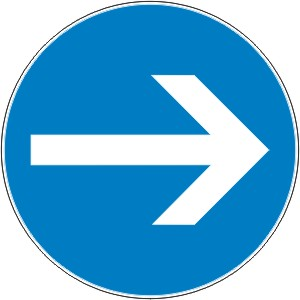
\includegraphics[scale=0.5]{figures/znak.png}
\caption{Prikaz korištenog znaka - obvezan smjer kretanja u desno}
\label{fig:znak}
\end{figure}

\begin{figure}[h]
\centering
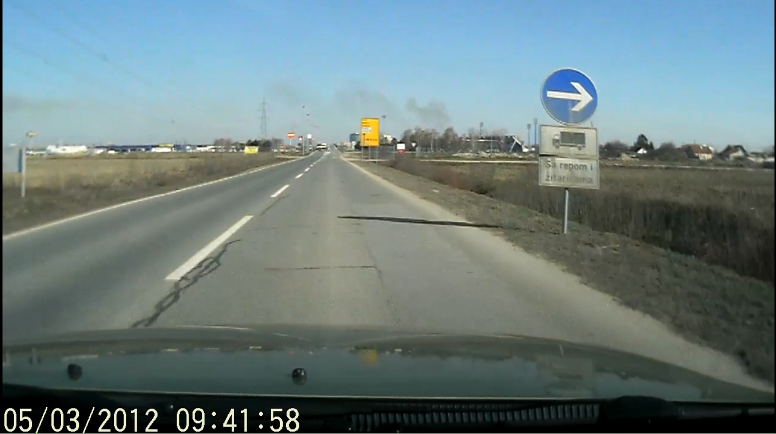
\includegraphics[scale=0.3]{figures/scena.png}
\caption{Prikaz testirane scene voznje}
\label{fig:scena.png}
\end{figure}

\subsection{Prikaz rezultata} % (fold)
\label{sub:Prikaz rezultata}

Rezultati su prikazani na slikama s dva prozora. U prvom prozoru 
prikazana je regija interesa sa scene unutar koje algoritmom
usporedbe tražimo znak. U drugom prozornu prikazana je matrica rezultata
koji algoritam koristi za pronalazak znaka. Postoji nekoliko tipova
rezultata: pozitivni, negativni, lažno pozitivni i lažno negativni.


\begin{figure}[h]
\centering
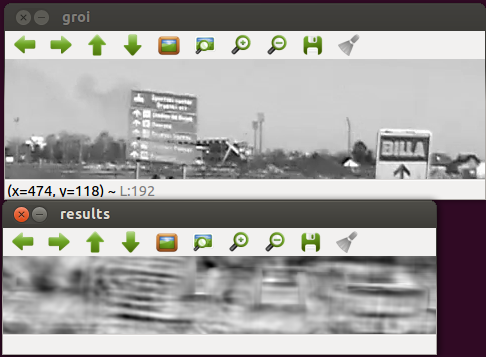
\includegraphics[scale=0.5]{figures/01.png}
\caption{}
\label{fig:01}
\end{figure}

% subsection Prikaz rezultata (end)
% section Rezultati (end)
